\section{Результаты классификации на чистых данных}
\label{sec:Chapter3}

В~данном разделе приводятся результаты обучения и~тестирования
трех моделей на~исходных, незашумленных данных.
Все~эксперименты воспроизводимы: фиксированы начальный номер
генератора случайных чисел (\texttt{random\_state=42}),
разбиение на~выборки и~гиперпараметры.

\subsection{Сводная таблица метрик}

Результаты на~тестовой выборке ($|\mathcal{D}_\text{test}| = 20\,005$)
представлены в~таблице~\ref{tab:clean_results}.

\begin{table}[h]
\centering
\caption{Метрики качества моделей на~чистых данных}
\label{tab:clean_results}
\begin{tabular}{lccc}
\hline
\textbf{Модель} & \textbf{Accuracy} & \textbf{Macro F1} & \textbf{Weighted F1} \\
\hline
1D~CNN      & \textbf{0.9917} & \textbf{0.9736} & \textbf{0.9918} \\
ResNet1D    & 0.9847          & 0.9532          & 0.9848          \\
RandomForest & 0.9848         & 0.9496          & 0.9841          \\
\hline
\end{tabular}
\end{table}

Все~три модели превышают порог Macro~F1~$\geq 0.90$,
поставленный в~разделе~\ref{sec:Chapter1}.
Наилучший результат демонстрирует 1D~CNN (Macro~F1~$= 0.974$),
опережая ResNet1D на~$0.020$ и~Random Forest на~$0.024$.
Несмотря на~то что~Accuracy у~RF и~ResNet1D практически одинакова
($0.9848$ против~$0.9847$), Macro~F1 у~ResNet1D выше
($0.9532$ против~$0.9496$) за~счет лучшей работы
с~миноритарными классами.

\subsection{Анализ по классам: матрицы ошибок}

\subsubsection{1D CNN}

\begin{figure}[h]
\centering
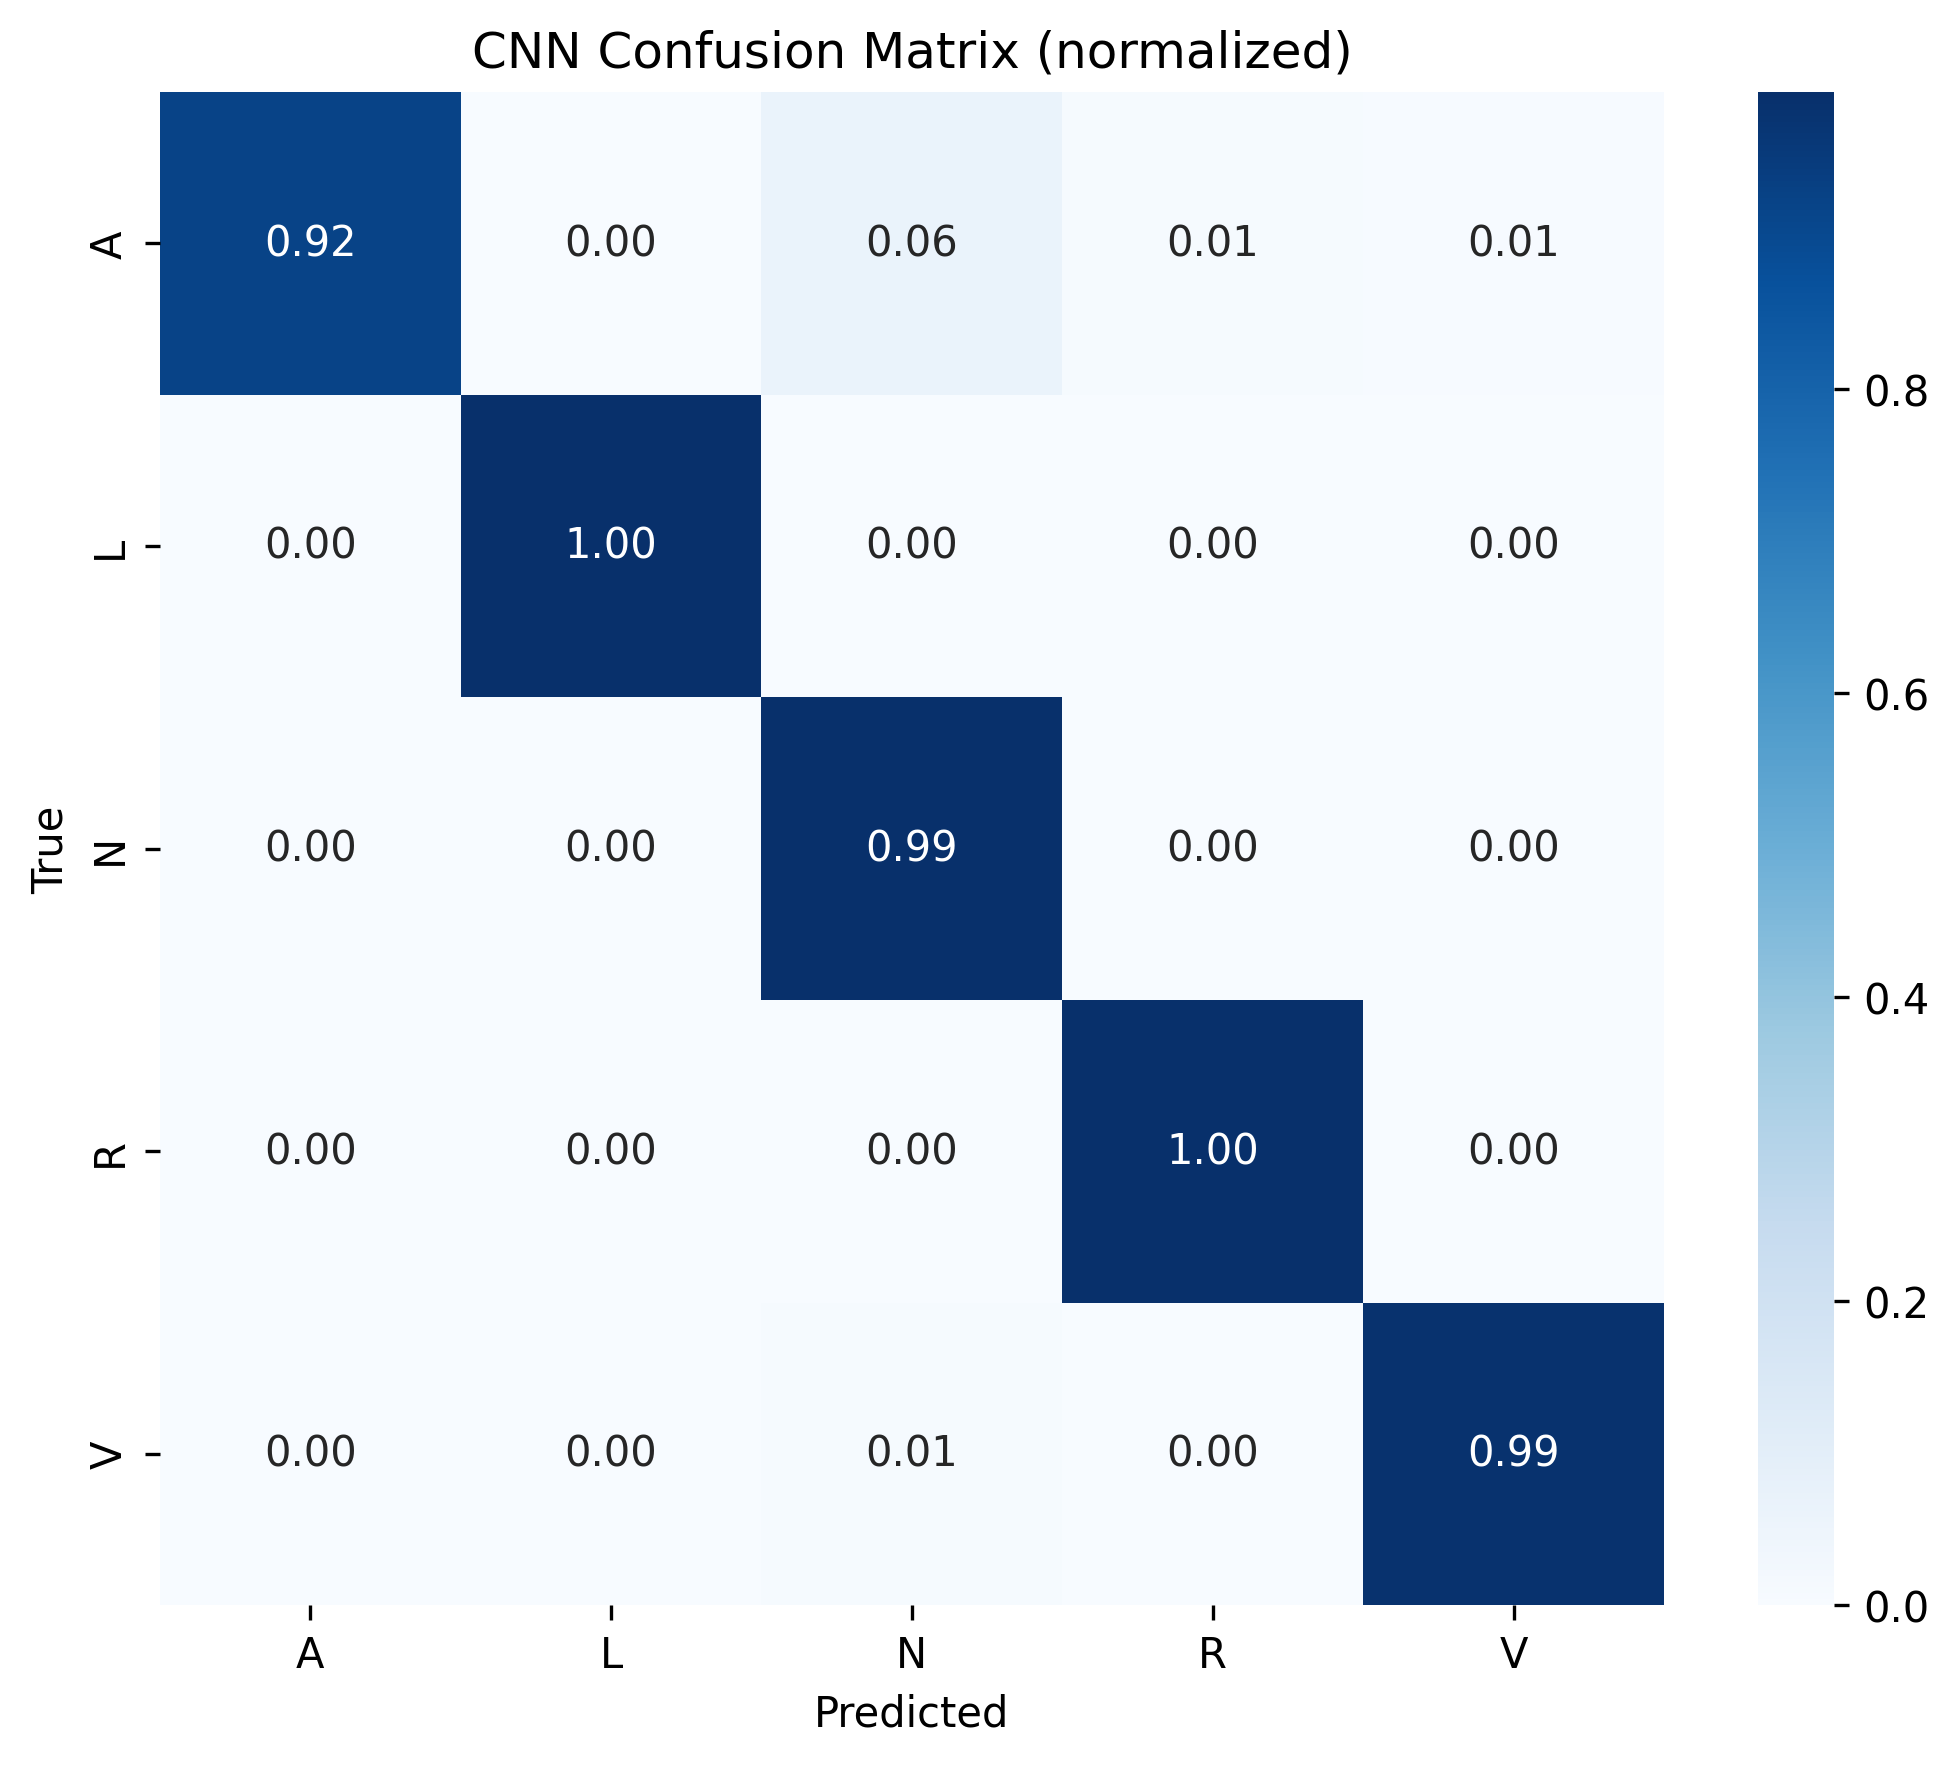
\includegraphics[width=0.65\textwidth]{../reports/figures/models/cm_cnn_normalized.png}
\caption{Нормализованная матрица ошибок 1D~CNN.
По диагонали~--- доля правильно классифицированных объектов каждого класса.}
\label{fig:cm_cnn}
\end{figure}

CNN добивается recall~$= 0.92$ для~класса~A~---
наилучший результат среди всех трех моделей.
Это достигается благодаря взвешенной функции потерь
(формула~\eqref{eq:wce}), которая увеличивает штраф
за~пропуск редких классов.
Классы~N, L, R распознаются практически безошибочно
(recall~$\geq 0.98$), класс~V~--- с~recall~$\approx 0.97$.

\subsubsection{ResNet1D}

\begin{figure}[h]
\centering
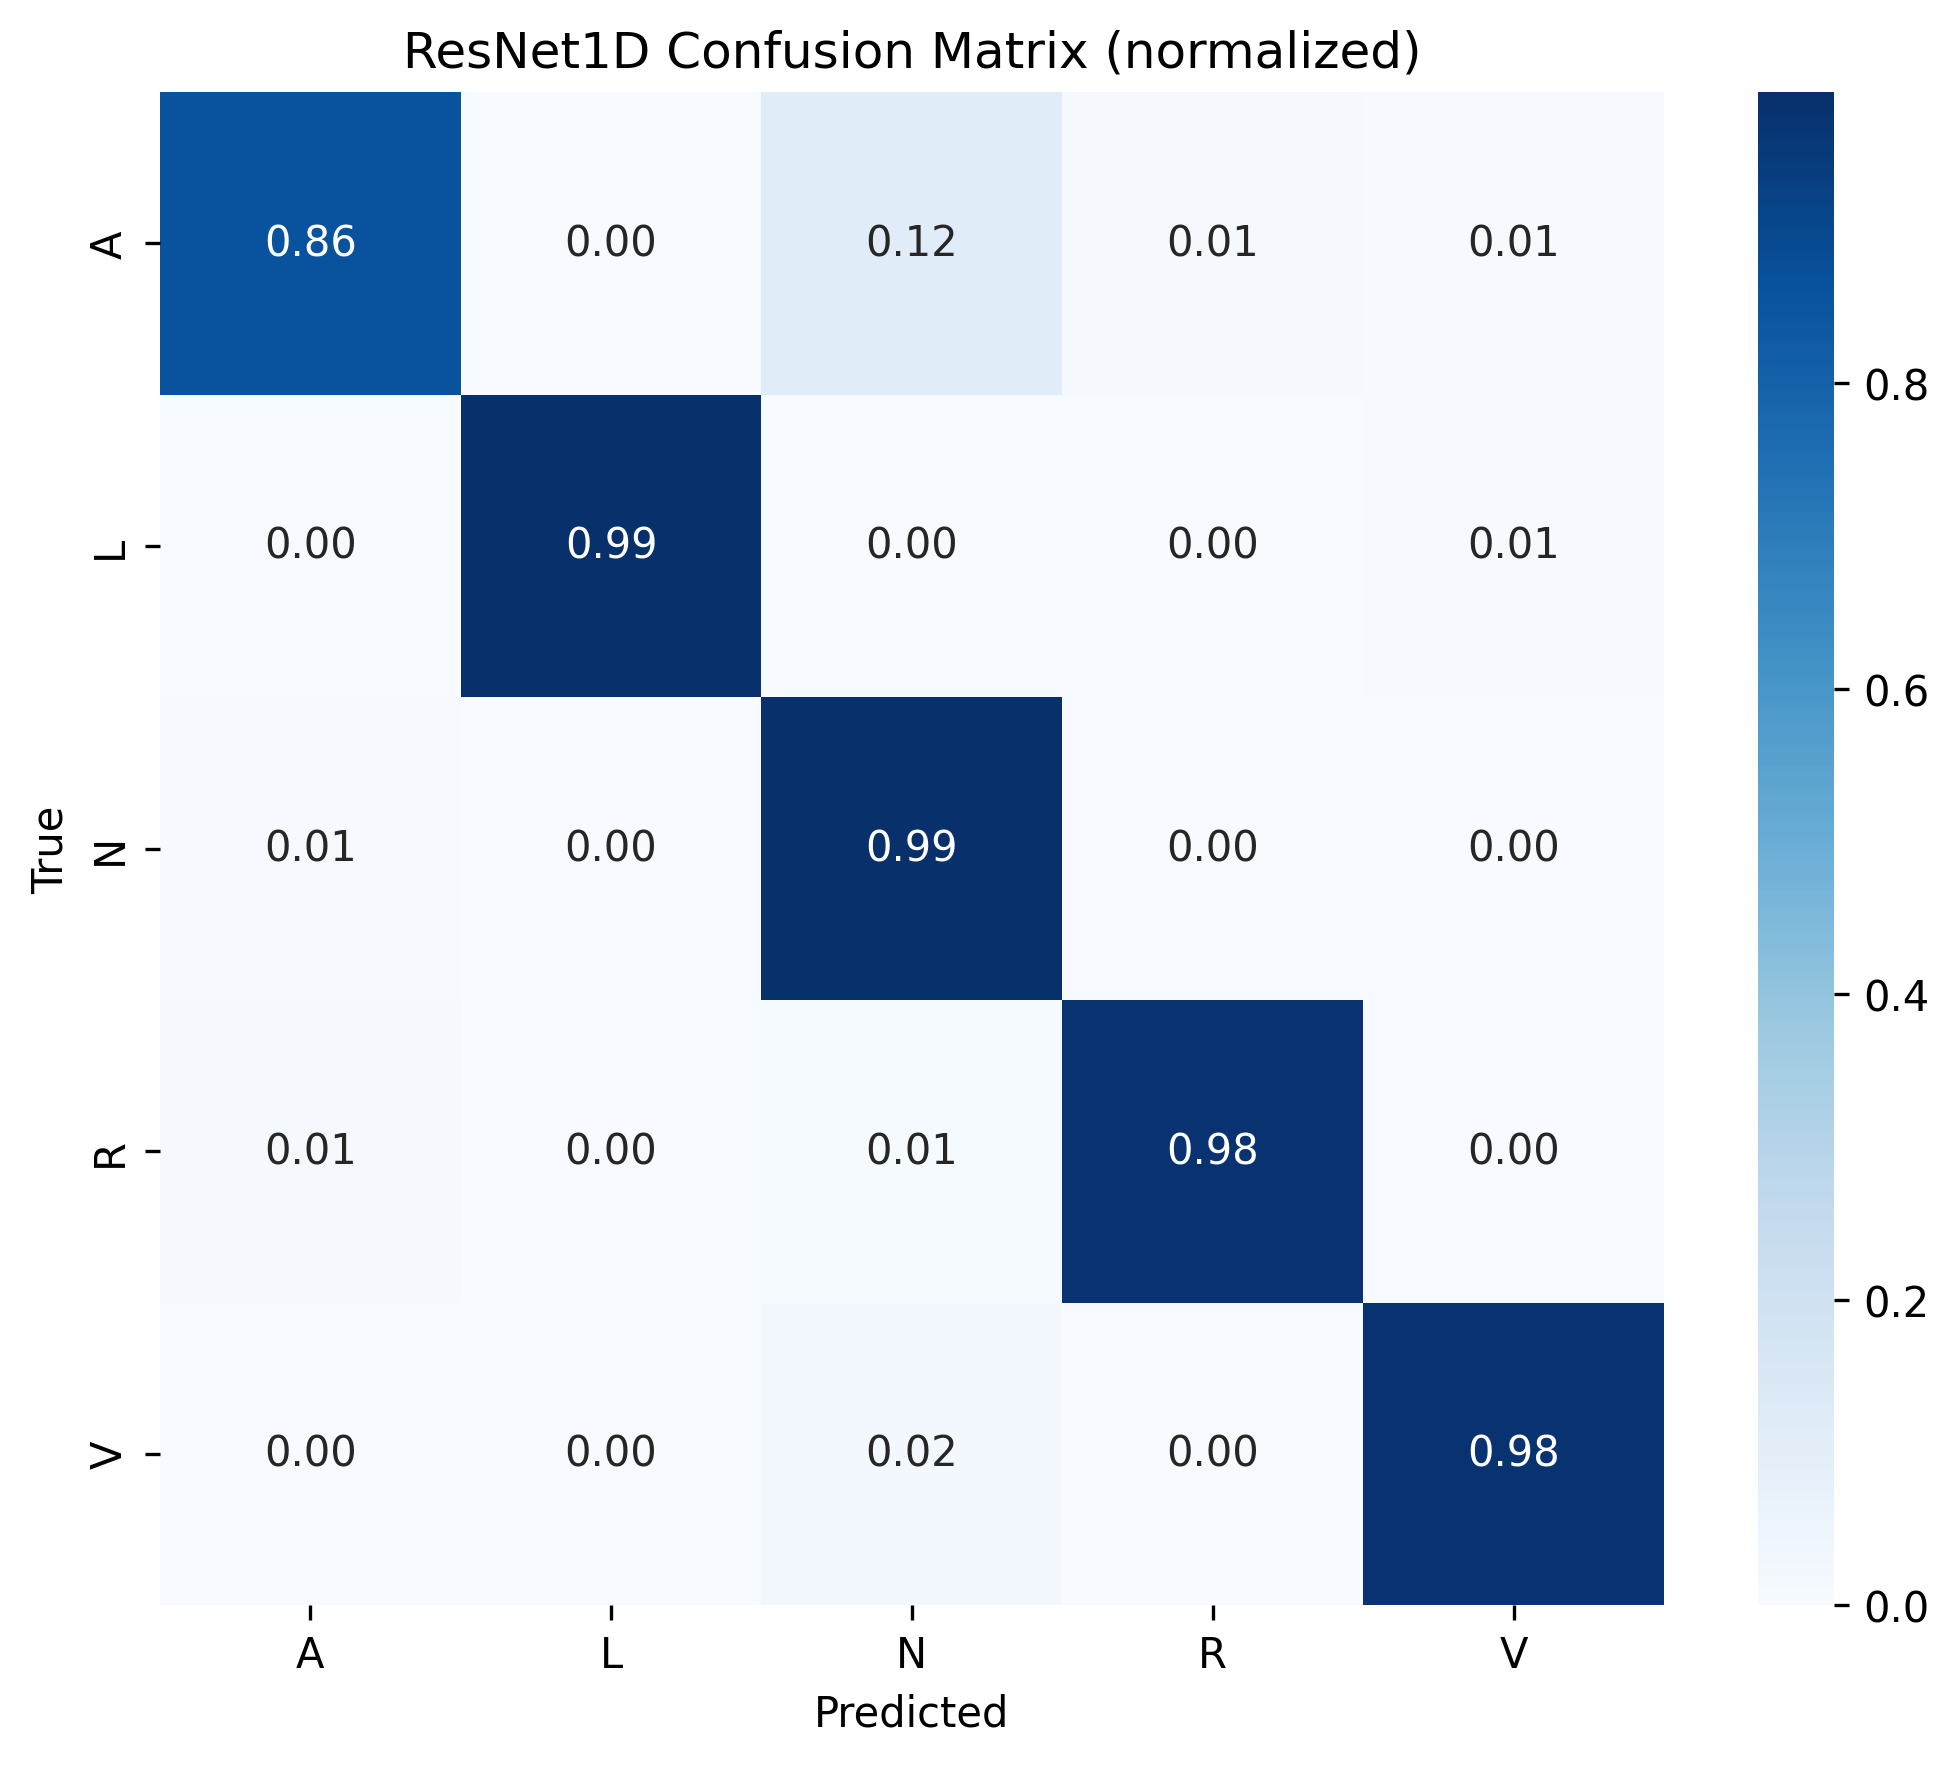
\includegraphics[width=0.65\textwidth]{../reports/figures/models/cm_resnet_normalized.png}
\caption{Нормализованная матрица ошибок ResNet1D.}
\label{fig:cm_resnet}
\end{figure}

ResNet1D устойчиво классифицирует классы~N, L, R, V
(recall~$\geq 0.94$).
Класс~A вызывает наибольшие затруднения: recall несколько ниже,
чем~у~CNN, что~объясняется меньшим числом эпох обучения
и~более сложной архитектурой, требующей большего времени сходимости.

\subsubsection{Random Forest}

\begin{figure}[h]
\centering
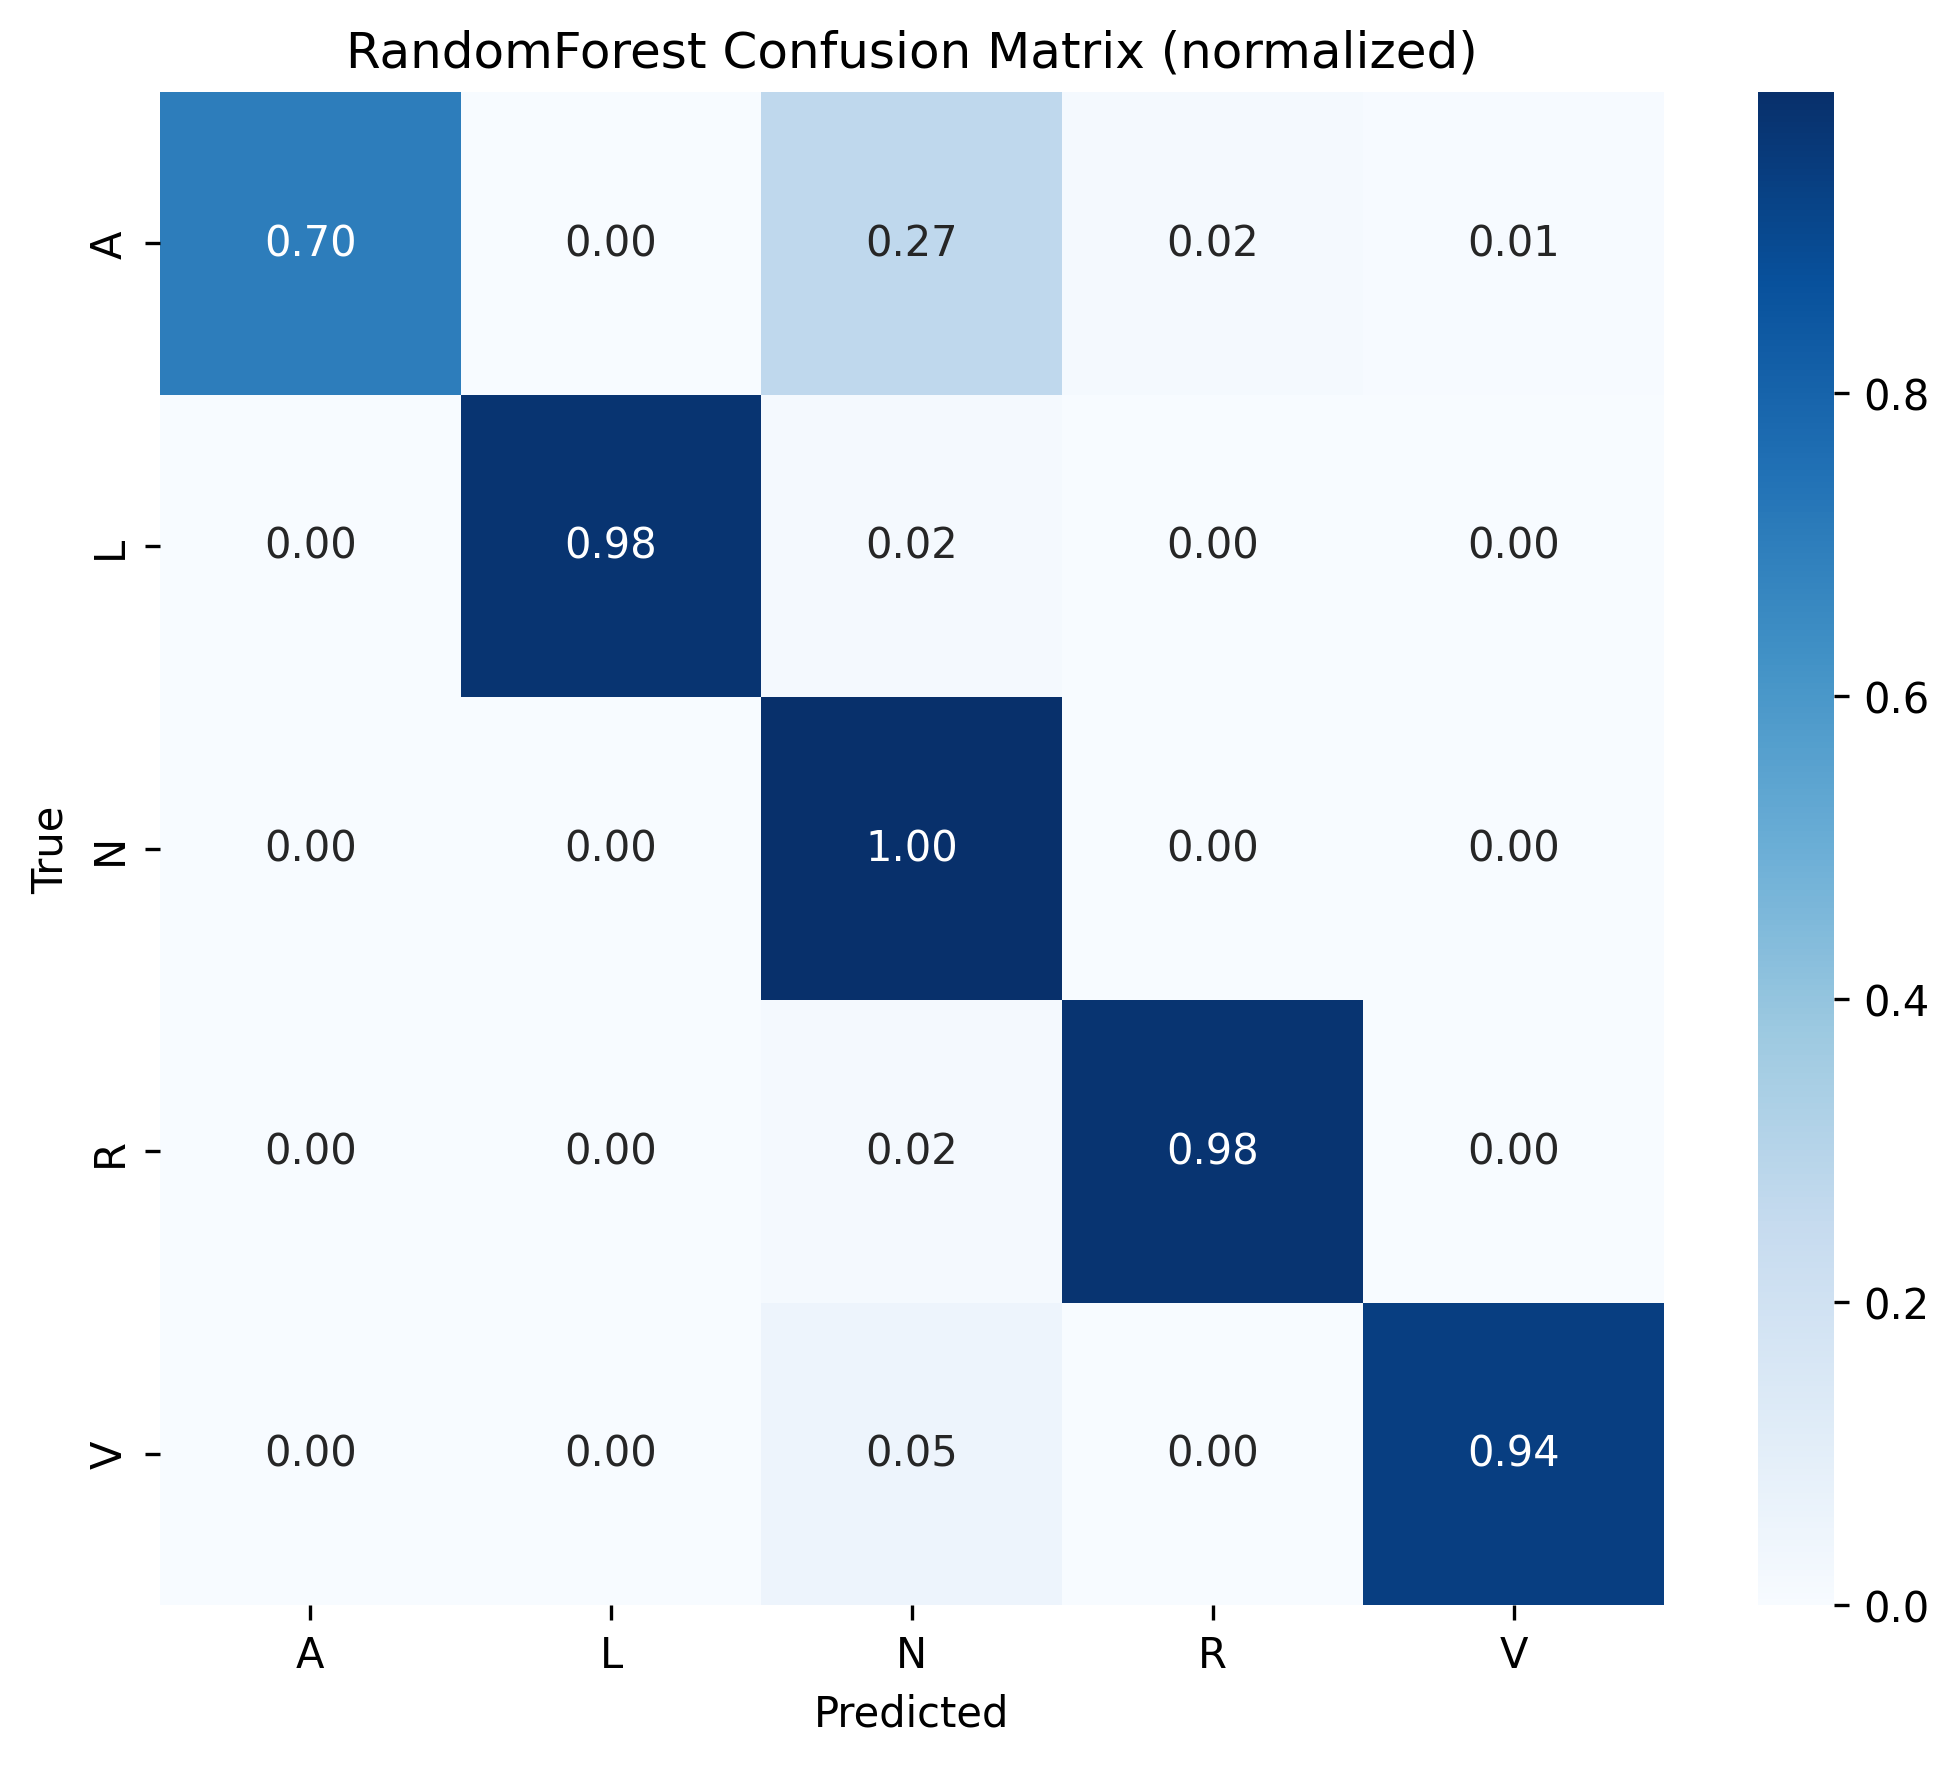
\includegraphics[width=0.65\textwidth]{../reports/figures/models/cm_rf_normalized.png}
\caption{Нормализованная матрица ошибок Random Forest.}
\label{fig:cm_rf}
\end{figure}

Главная слабость RF~--- recall класса~A~$= 0.70$:
каждый третий случай предсердной экстрасистолы пропускается.
Это существенный недостаток с~клинической точки зрения.
Стратегия \texttt{balanced\_subsample} частично компенсирует
дисбаланс, однако не~дает того эффекта, что~явное
взвешивание функции потерь у~нейронных сетей.
Классы~L, R, N распознаются надежно (recall~$\geq 0.98$).

\subsubsection{Сравнение по классу A}

Таблица~\ref{tab:class_a} обобщает результаты для~наиболее
проблематичного класса~A~--- предсердной экстрасистолы.

\begin{table}[h]
\centering
\caption{Метрики для класса A (предсердная экстрасистола)}
\label{tab:class_a}
\begin{tabular}{lcccc}
\hline
\textbf{Модель} & \textbf{Precision} & \textbf{Recall} &
\textbf{F1} & \textbf{Поддержка} \\
\hline
1D~CNN       & 0.96 & \textbf{0.92} & \textbf{0.94} & 509 \\
ResNet1D     & 0.95 & 0.88          & 0.91          & 509 \\
RandomForest & 0.98 & 0.70          & 0.82          & 509 \\
\hline
\end{tabular}
\end{table}

Все~модели удовлетворяют требованию recall(A)~$\geq 0.65$
из~постановки задачи (раздел~\ref{sec:Chapter1}).
CNN превышает этот порог с~запасом в~$0.27$.

\subsection{Кривые обучения нейронных сетей}

\subsubsection{1D CNN}

\begin{figure}[h]
\centering
\begin{minipage}{0.48\textwidth}
    \centering
    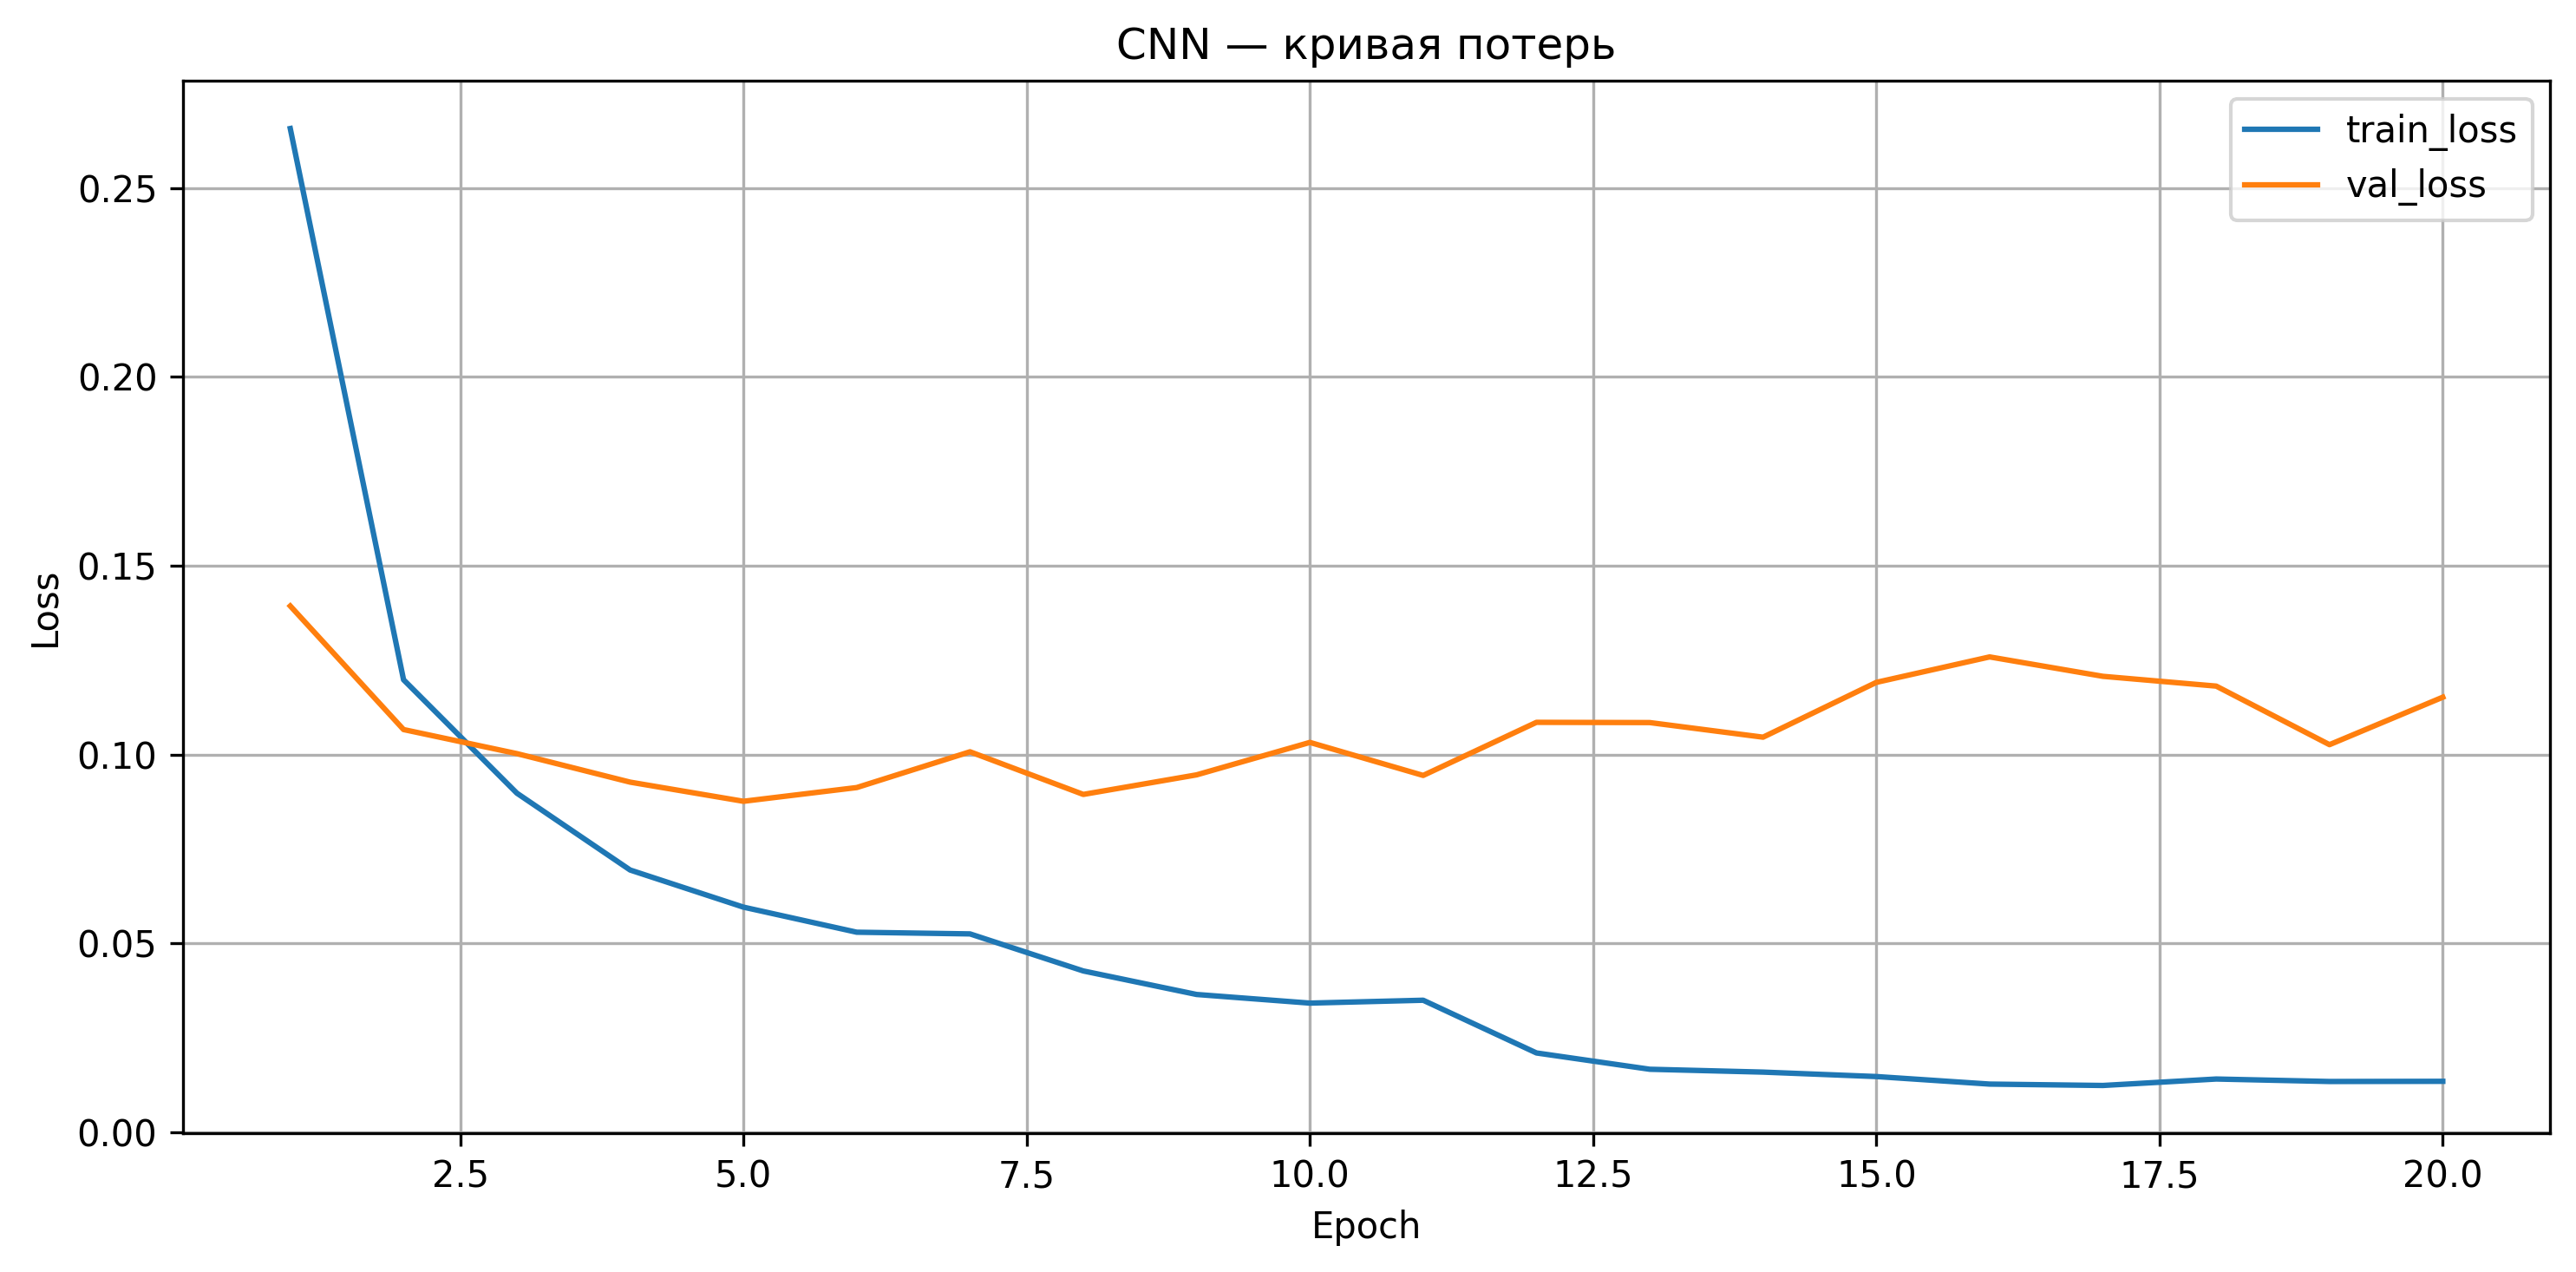
\includegraphics[width=\textwidth]{../reports/figures/models/cnn_loss_curve.png}
\end{minipage}
\hfill
\begin{minipage}{0.48\textwidth}
    \centering
    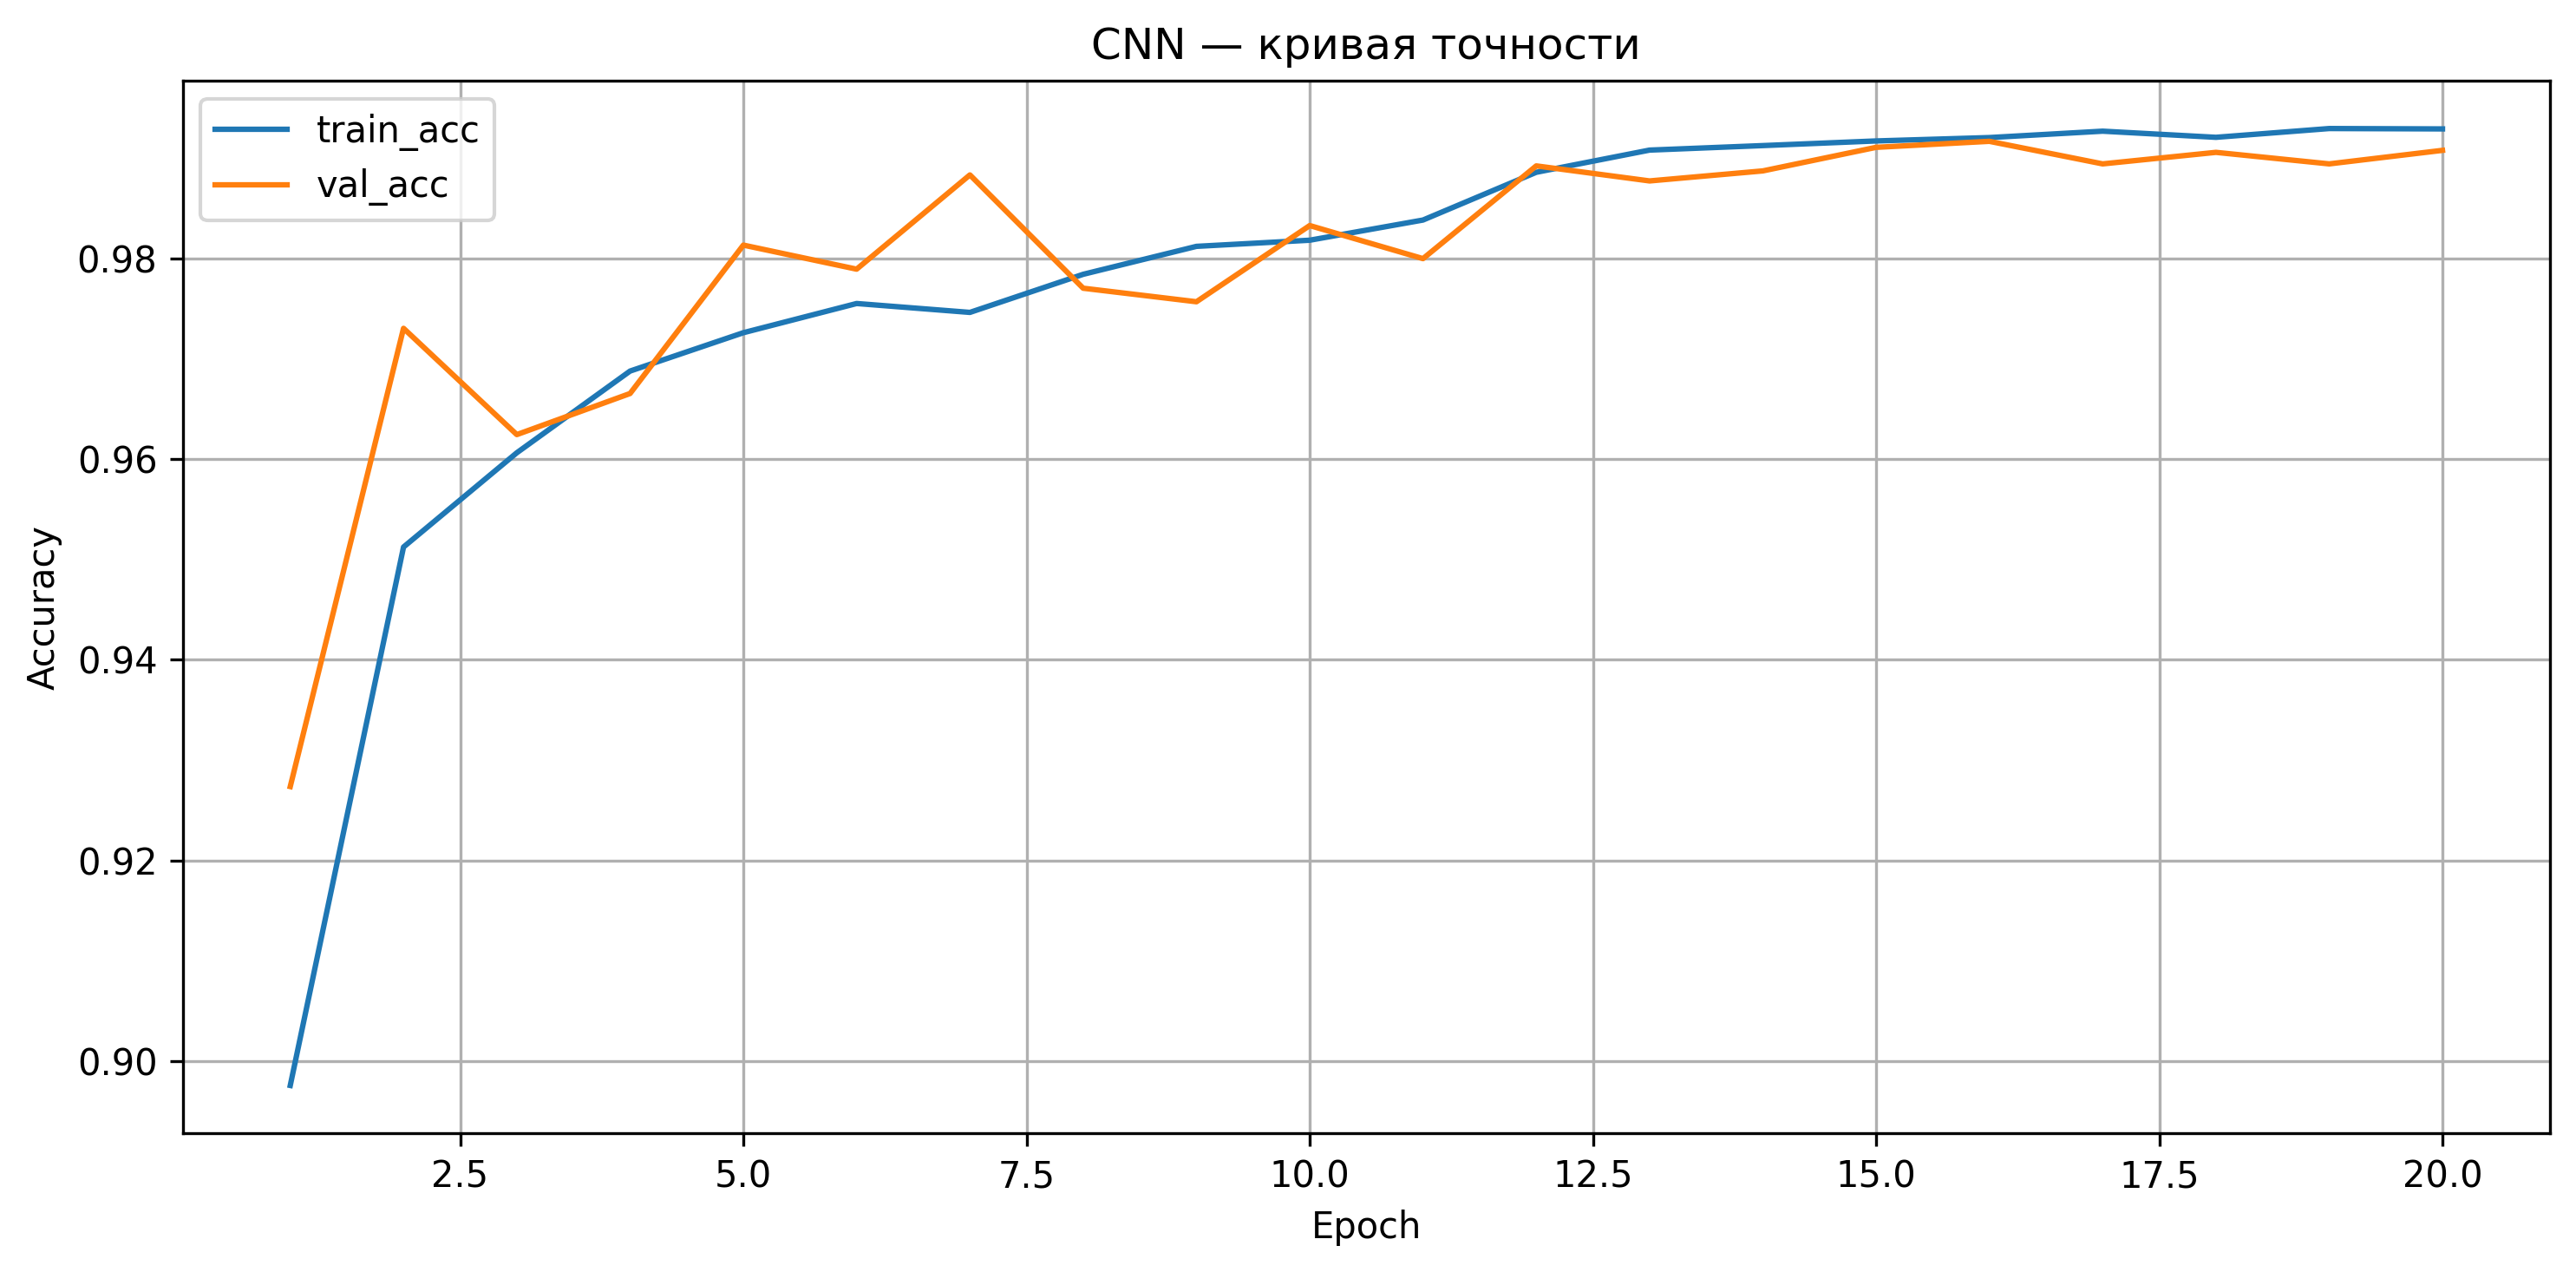
\includegraphics[width=\textwidth]{../reports/figures/models/cnn_accuracy_curve.png}
\end{minipage}
\caption{Кривые потерь (слева) и~точности (справа) 1D~CNN
в~процессе обучения. Вертикальная линия соответствует эпохе
ранней остановки.}
\label{fig:cnn_curves}
\end{figure}

Сеть сходится равномерно: валидационная и~обучающая кривые
идут вместе~--- признак отсутствия переобучения.
Механизм ReduceLROnPlateau снижает скорость обучения примерно
на~$10$--$12$~эпохе, что~проявляется в~характерном «перегибе»
кривой потерь.
Ранняя остановка фиксирует лучшие веса до~начала возможного
переобучения.

\subsubsection{ResNet1D}

\begin{figure}[h]
\centering
\begin{minipage}{0.48\textwidth}
    \centering
    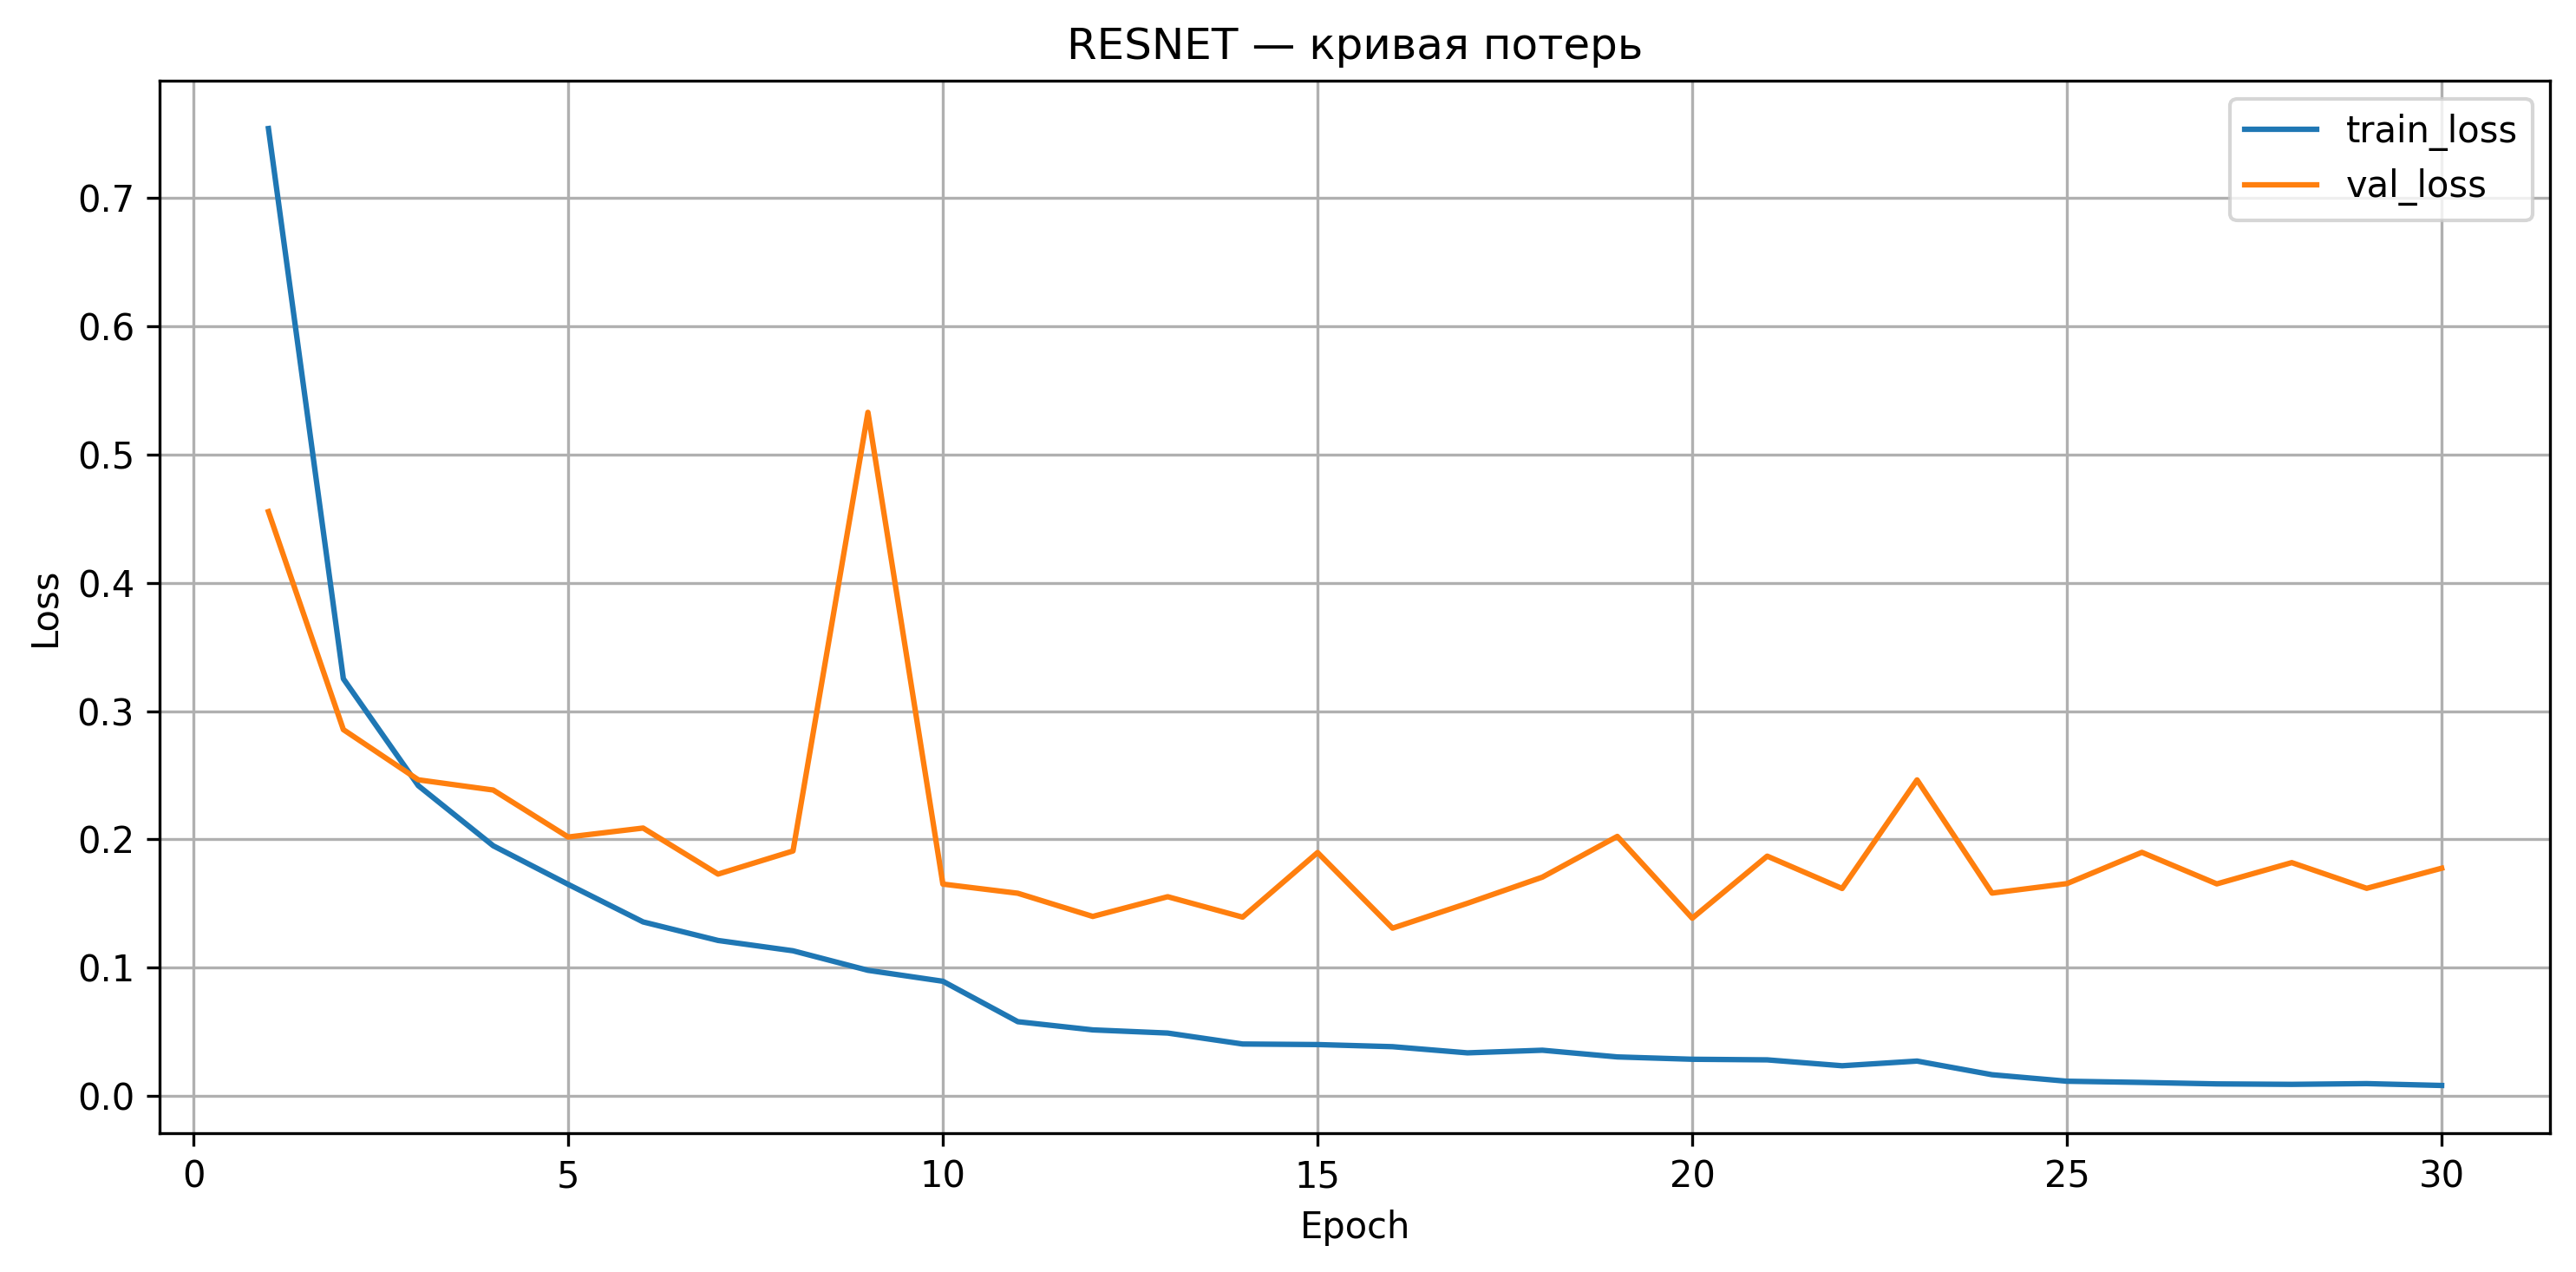
\includegraphics[width=\textwidth]{../reports/figures/models/resnet_loss_curve.png}
\end{minipage}
\hfill
\begin{minipage}{0.48\textwidth}
    \centering
    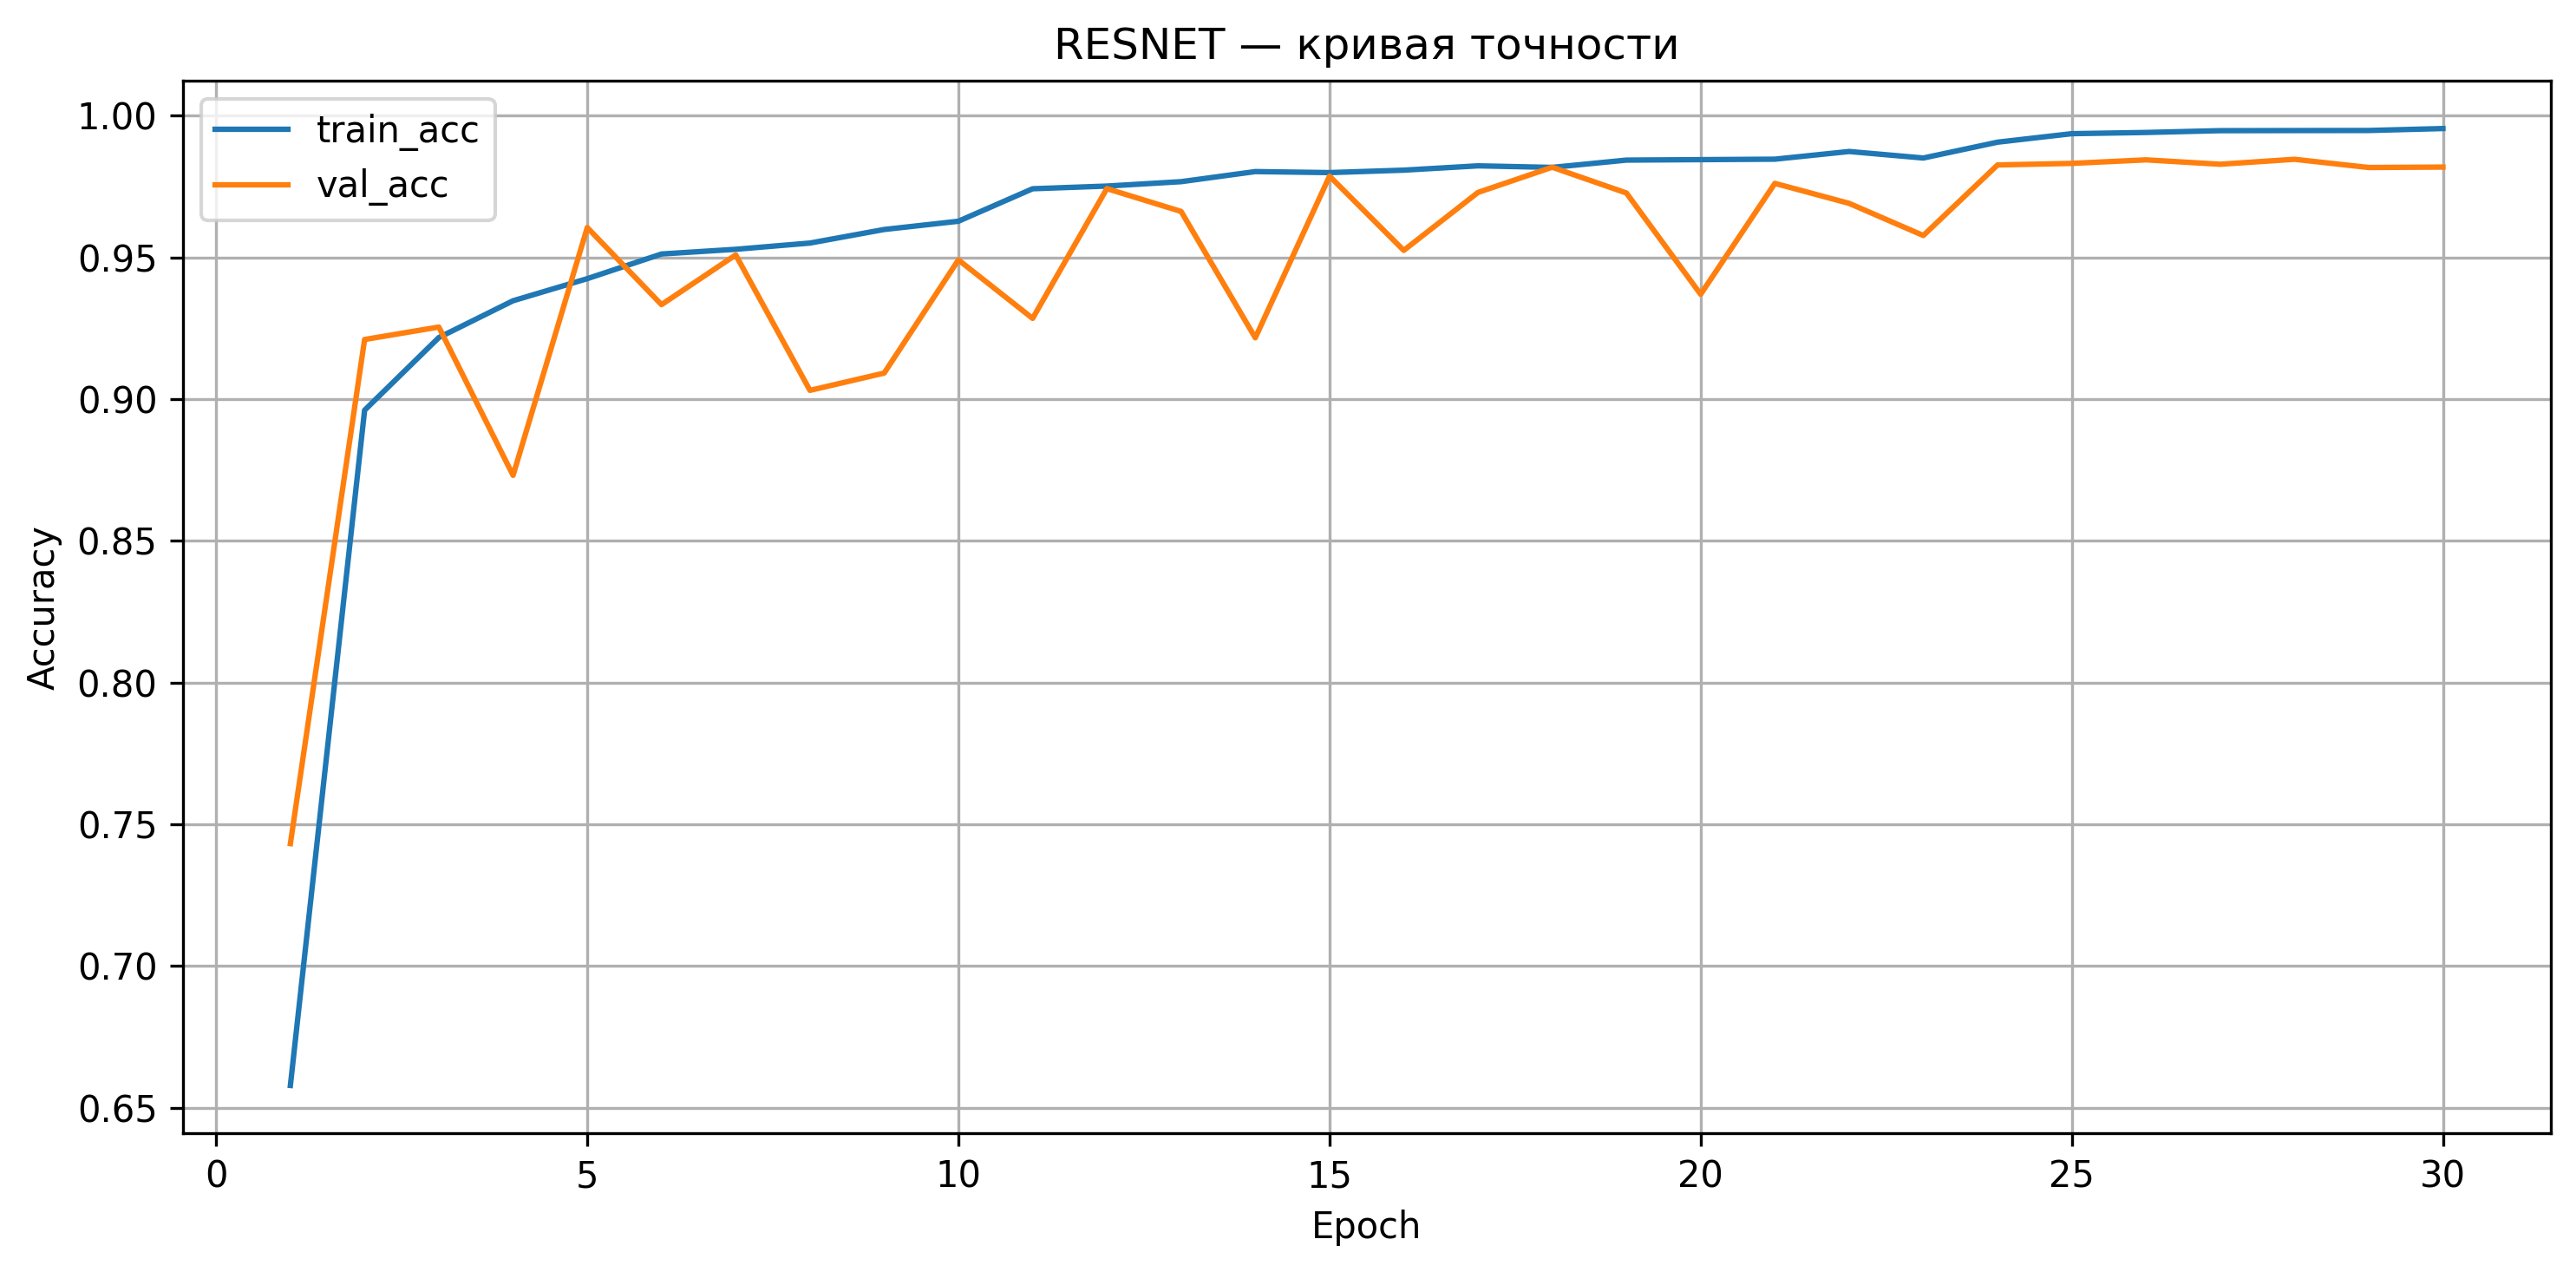
\includegraphics[width=\textwidth]{../reports/figures/models/resnet_accuracy_curve.png}
\end{minipage}
\caption{Кривые потерь и~точности ResNet1D.}
\label{fig:resnet_curves}
\end{figure}

ResNet1D требует больше эпох для~стабилизации по~сравнению
с~CNN, что~характерно для~более глубоких архитектур:
веса нескольких остаточных блоков должны согласоваться
друг~с~другом.
Остаточные соединения обеспечивают монотонное снижение потерь
без~«провалов», характерных для~сетей без~skip-connections.

\subsection{Важность признаков Random Forest}

\begin{figure}[h]
\centering
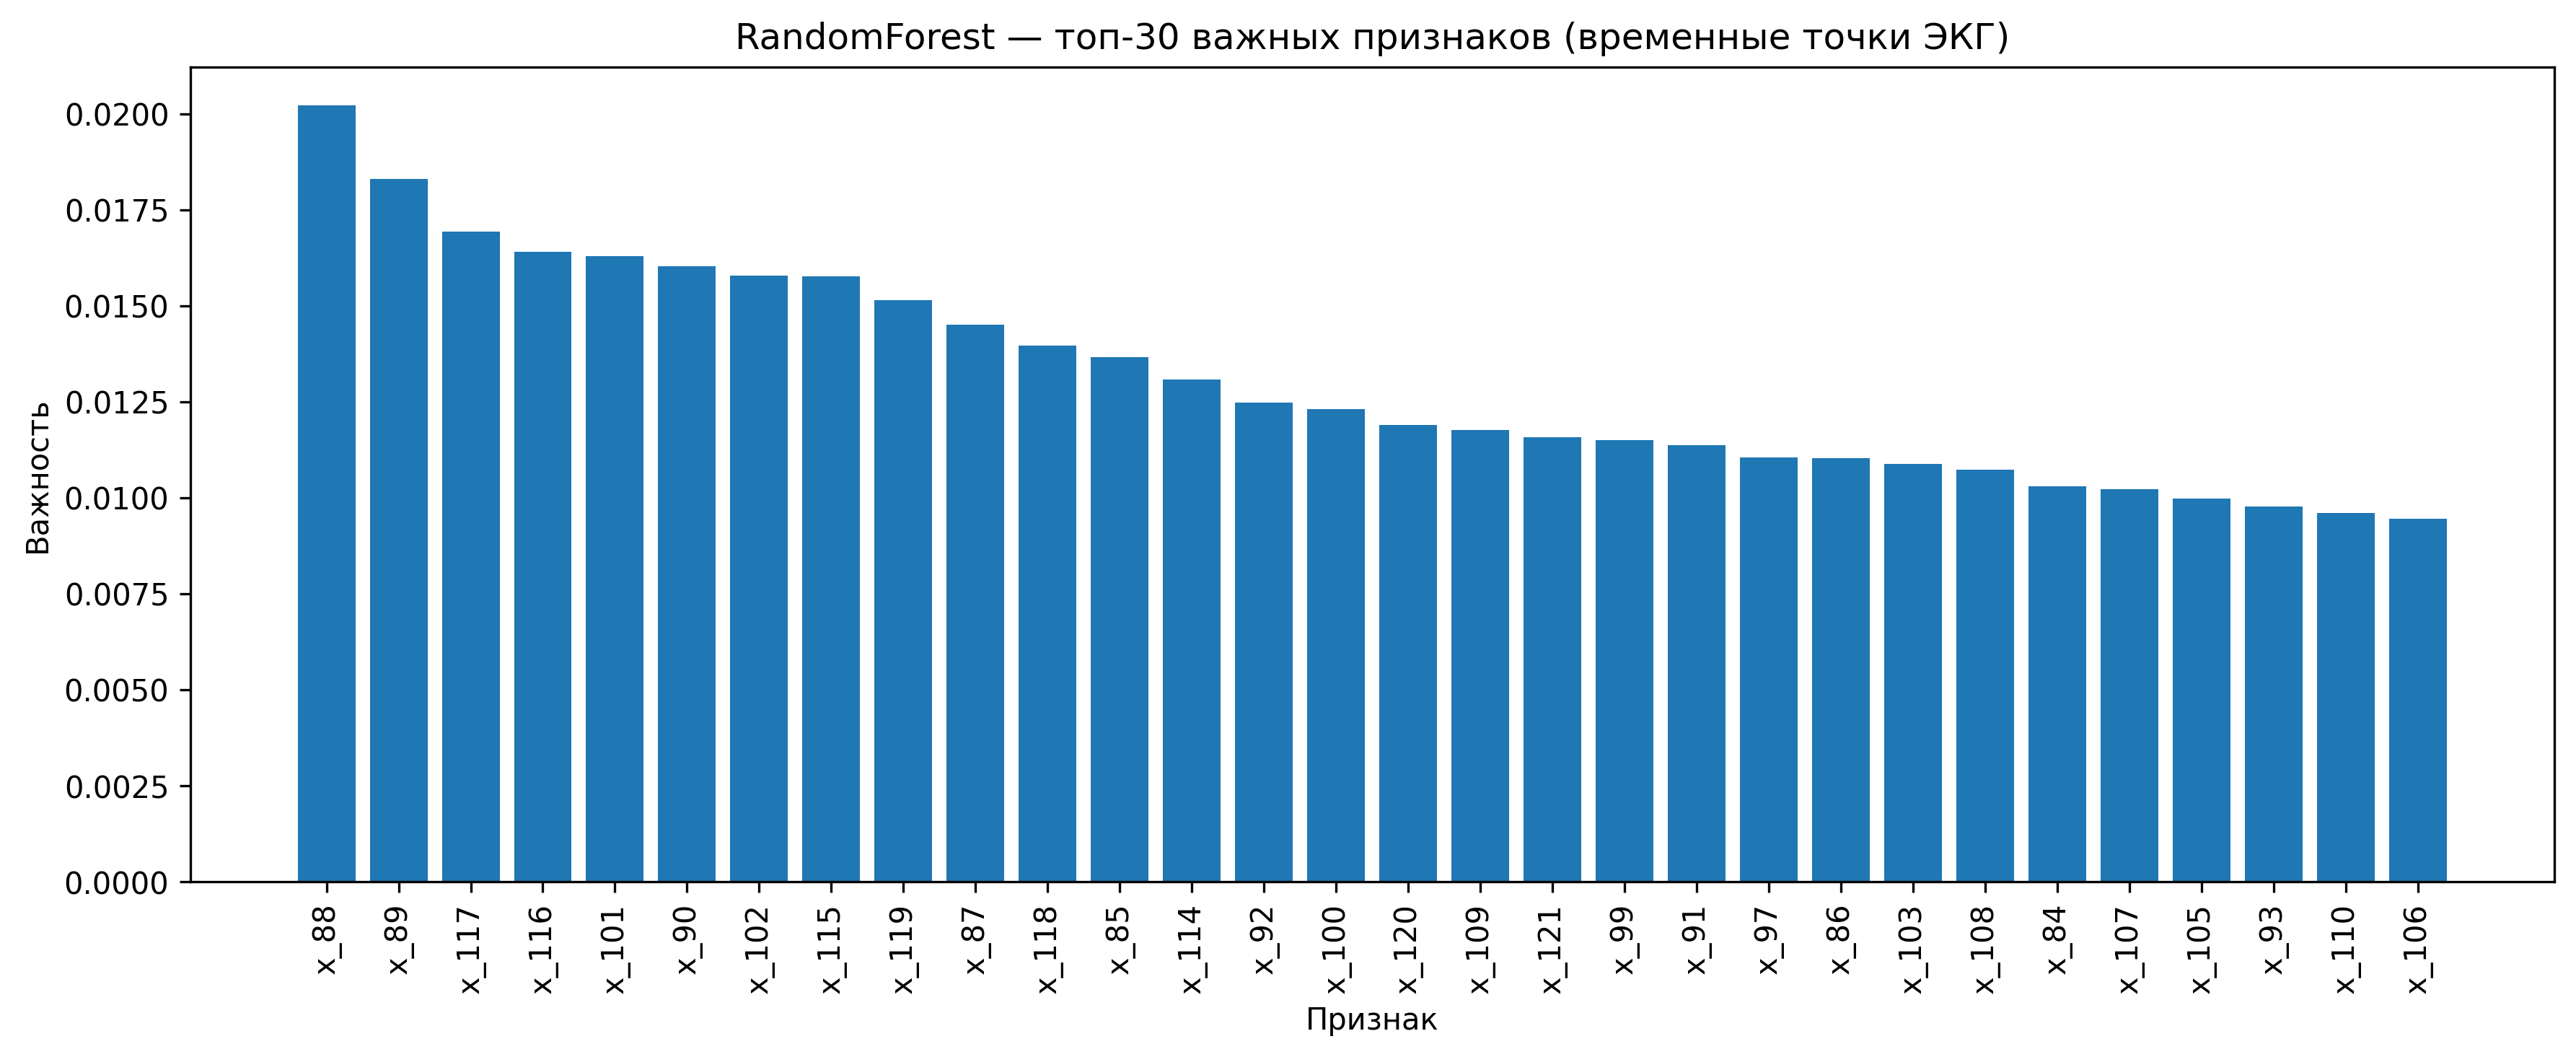
\includegraphics[width=\textwidth]{../reports/figures/models/rf_feature_importance.png}
\caption{Топ-30 наиболее важных временны\'{х} точек для~Random Forest
(оценка MDI).
По оси абсцисс~--- индекс отсчета в~окне $[x_0,\ldots,x_{239}]$;
по~оси ординат~--- нормированная важность.}
\label{fig:rf_importance}
\end{figure}

Наиболее информативными оказываются отсчеты в~диапазоне
$x_{95}$--$x_{115}$~--- непосредственно вблизи R-пика
(который находится в~позиции $x_{100}$).
Это соответствует крутому подъему и~спаду комплекса~QRS~---
наиболее характерному признаку для~разделения желудочковых
(V) и~предсердных (A) аномалий.
Отсчеты, соответствующие зубцу~T ($x_{140}$--$x_{200}$),
занимают второй по~значимости диапазон: форма~T-волны
дифференцирует блокады левой и~правой ножек (L~и~R).

\subsection{Эксперимент с вейвлет-признаками}

\begin{figure}[h]
\centering
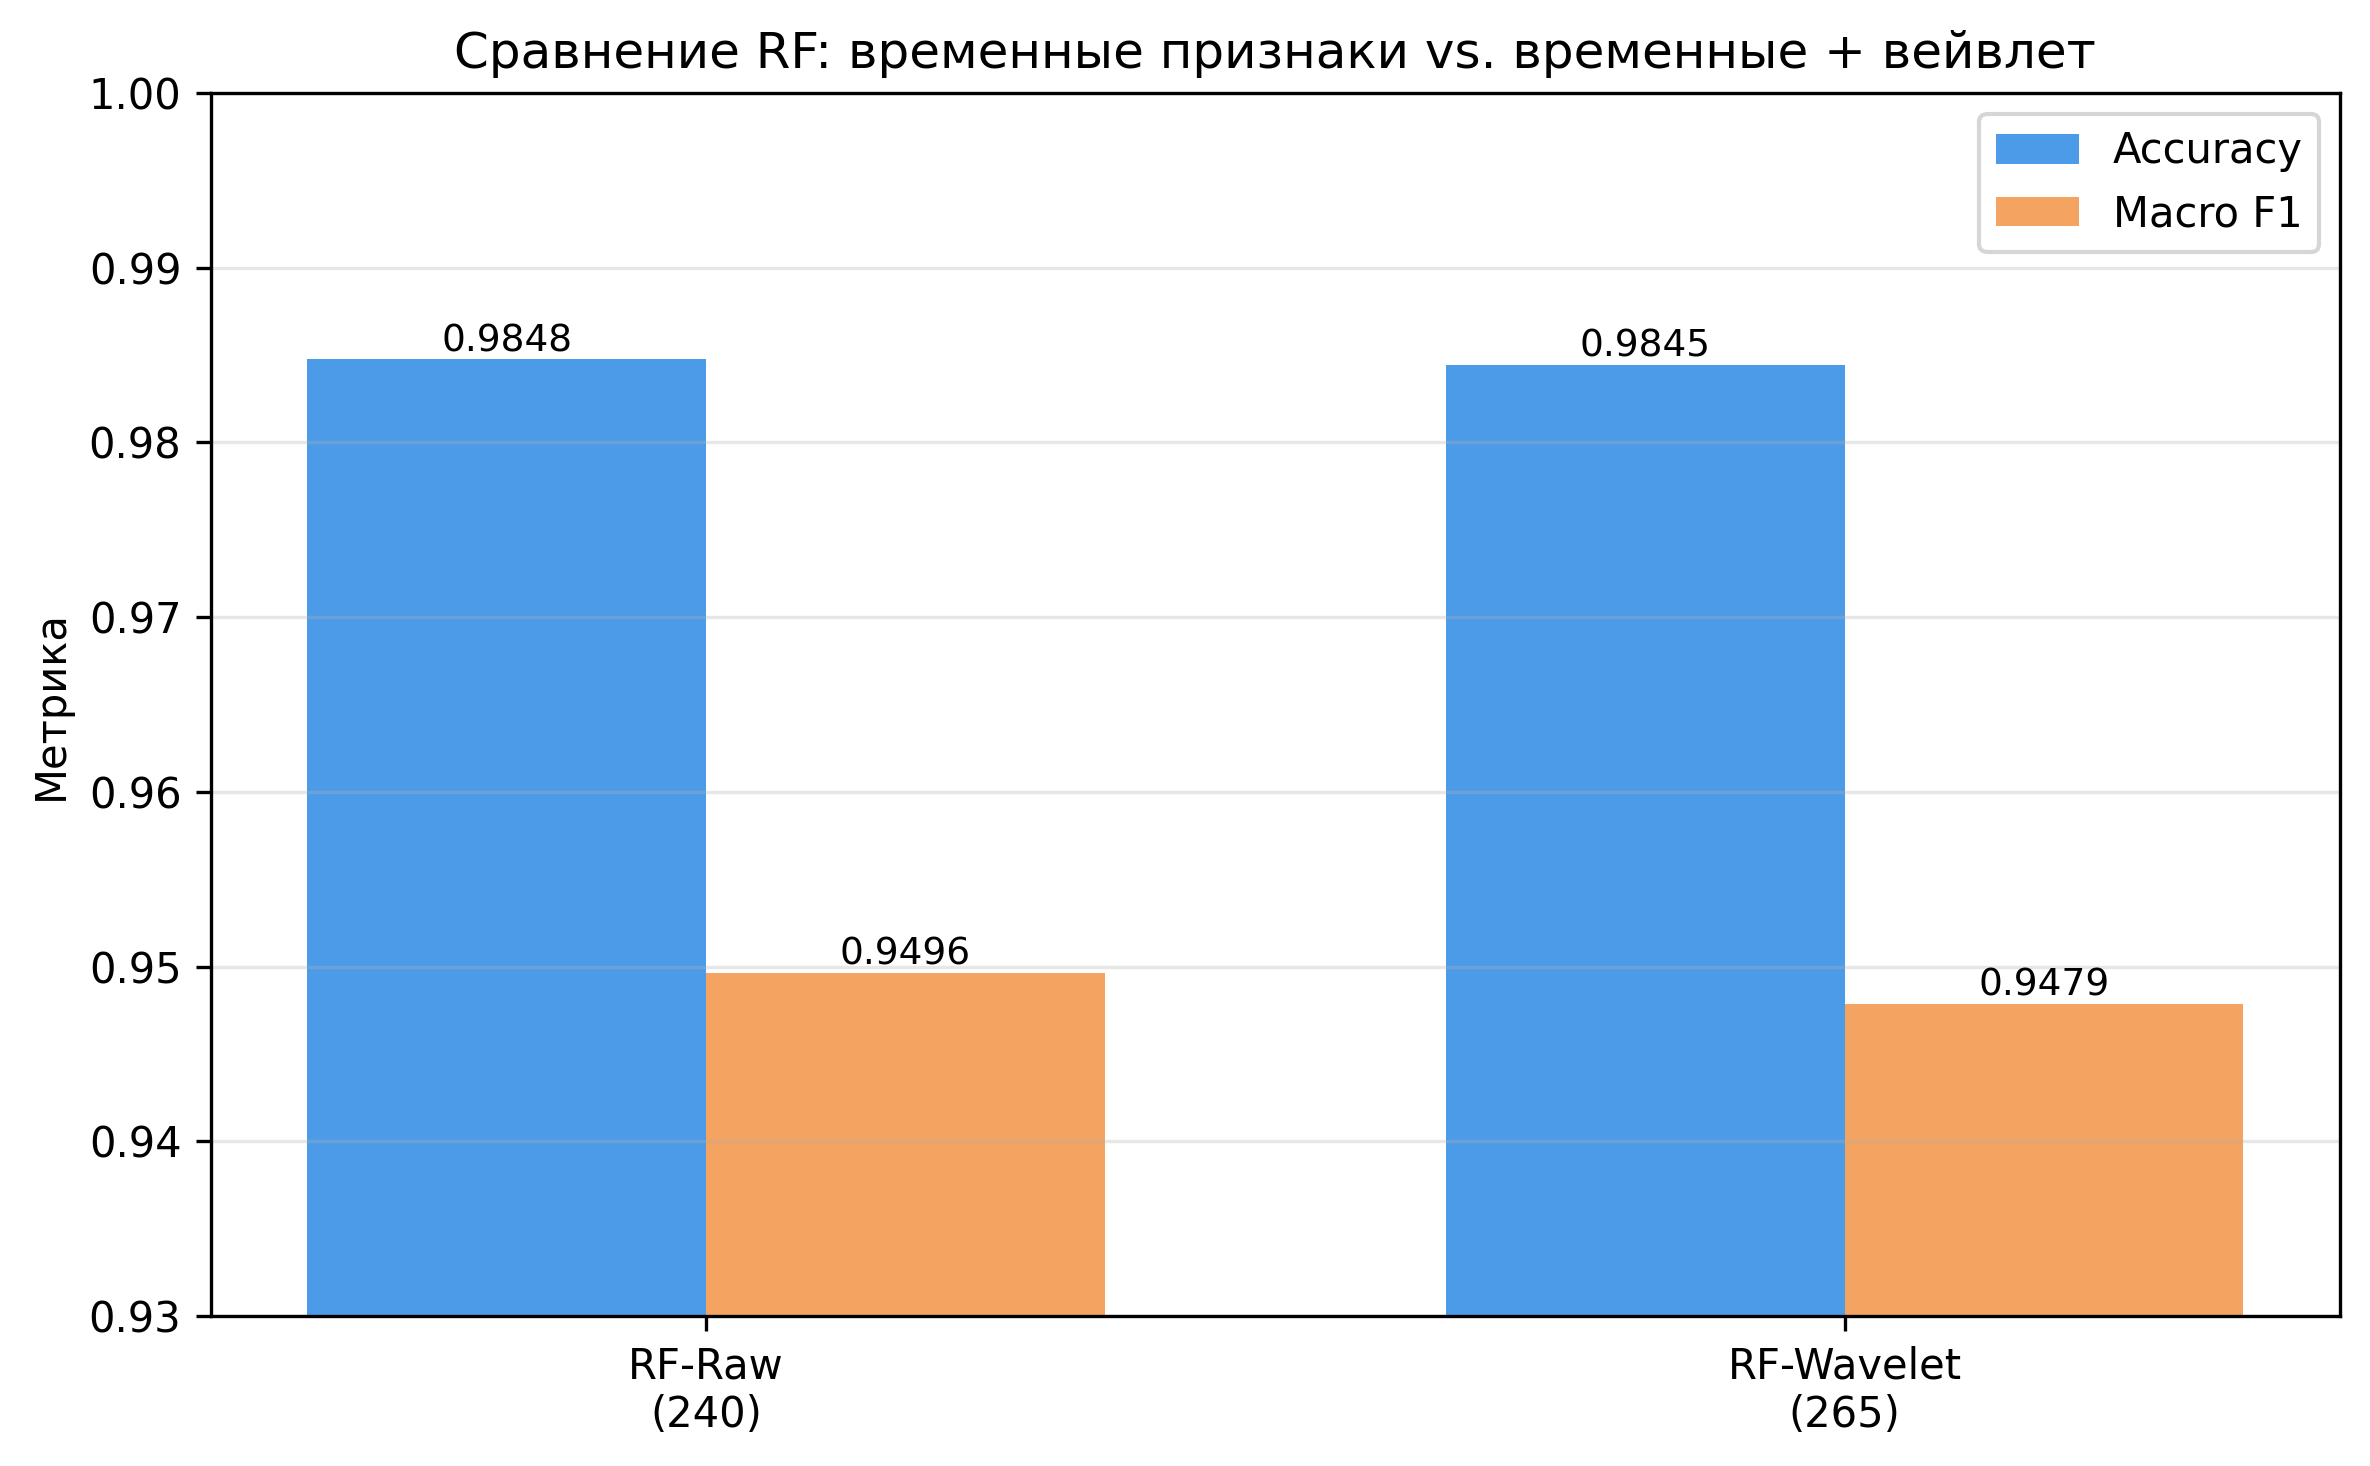
\includegraphics[width=0.75\textwidth]{../reports/figures/models/rf_wavelet_vs_raw_comparison.png}
\caption{Сравнение RF на~сырых признаках (240~отсчетов)
и~расширенных вейвлет-признаках (265~признаков).}
\label{fig:rf_wavelet_comp}
\end{figure}

Добавление $25$ вейвлет-признаков (ДВП db4, 4~уровня)
к~$240$ временны\'{м} отсчетам не~улучшило качество RF:
Macro~F1~$= 0.9479$ против~$0.9496$ (таблица~\ref{tab:wavelet_exp}).

\begin{table}[h]
\centering
\caption{Результаты эксперимента с вейвлет-признаками}
\label{tab:wavelet_exp}
\begin{tabular}{lcccc}
\hline
\textbf{Модель} & \textbf{Признаков} & \textbf{Accuracy} &
\textbf{Macro F1} & \textbf{Weighted F1} \\
\hline
RF-Raw     & 240 & 0.9848 & \textbf{0.9496} & 0.9841 \\
RF-Wavelet & 265 & 0.9845 & 0.9479          & 0.9837 \\
\hline
\end{tabular}
\end{table}

Разница Macro~F1~$= -0.0017$ находится в~пределах статистической
погрешности (для~выборки 20\,005~объектов оценка дисперсии
F1-меры невелика, однако систематического улучшения нет).
Вероятная причина: случайный лес на~$240$~сырых отсчетах
уже~неявно извлекает частотно-временны\'{е} паттерны~---
в~частности, разность соседних отсчетов кодирует локальную
производную, а~значит, и~высокочастотные компоненты.
Агрегатные статистики~($\bar{c},\,\sigma,\,E$) по~каждой
подполосе, напротив, теряют позиционную информацию.

Важность групп признаков (рисунок~\ref{fig:wt_imp}) показывает,
что~суммарный вклад $240$ временны\'{х} точек значительно
превышает суммарный вклад всех $25$ вейвлет-признаков.
Среди вейвлет-подполос наибольший вклад вносят $\mathrm{cD}_3$
и~$\mathrm{cD}_4$, соответствующие диапазону $11$--$45$~Гц,~---
именно там сосредоточена энергия комплекса~QRS и~зубцов~P, T.

\begin{figure}[h]
\centering
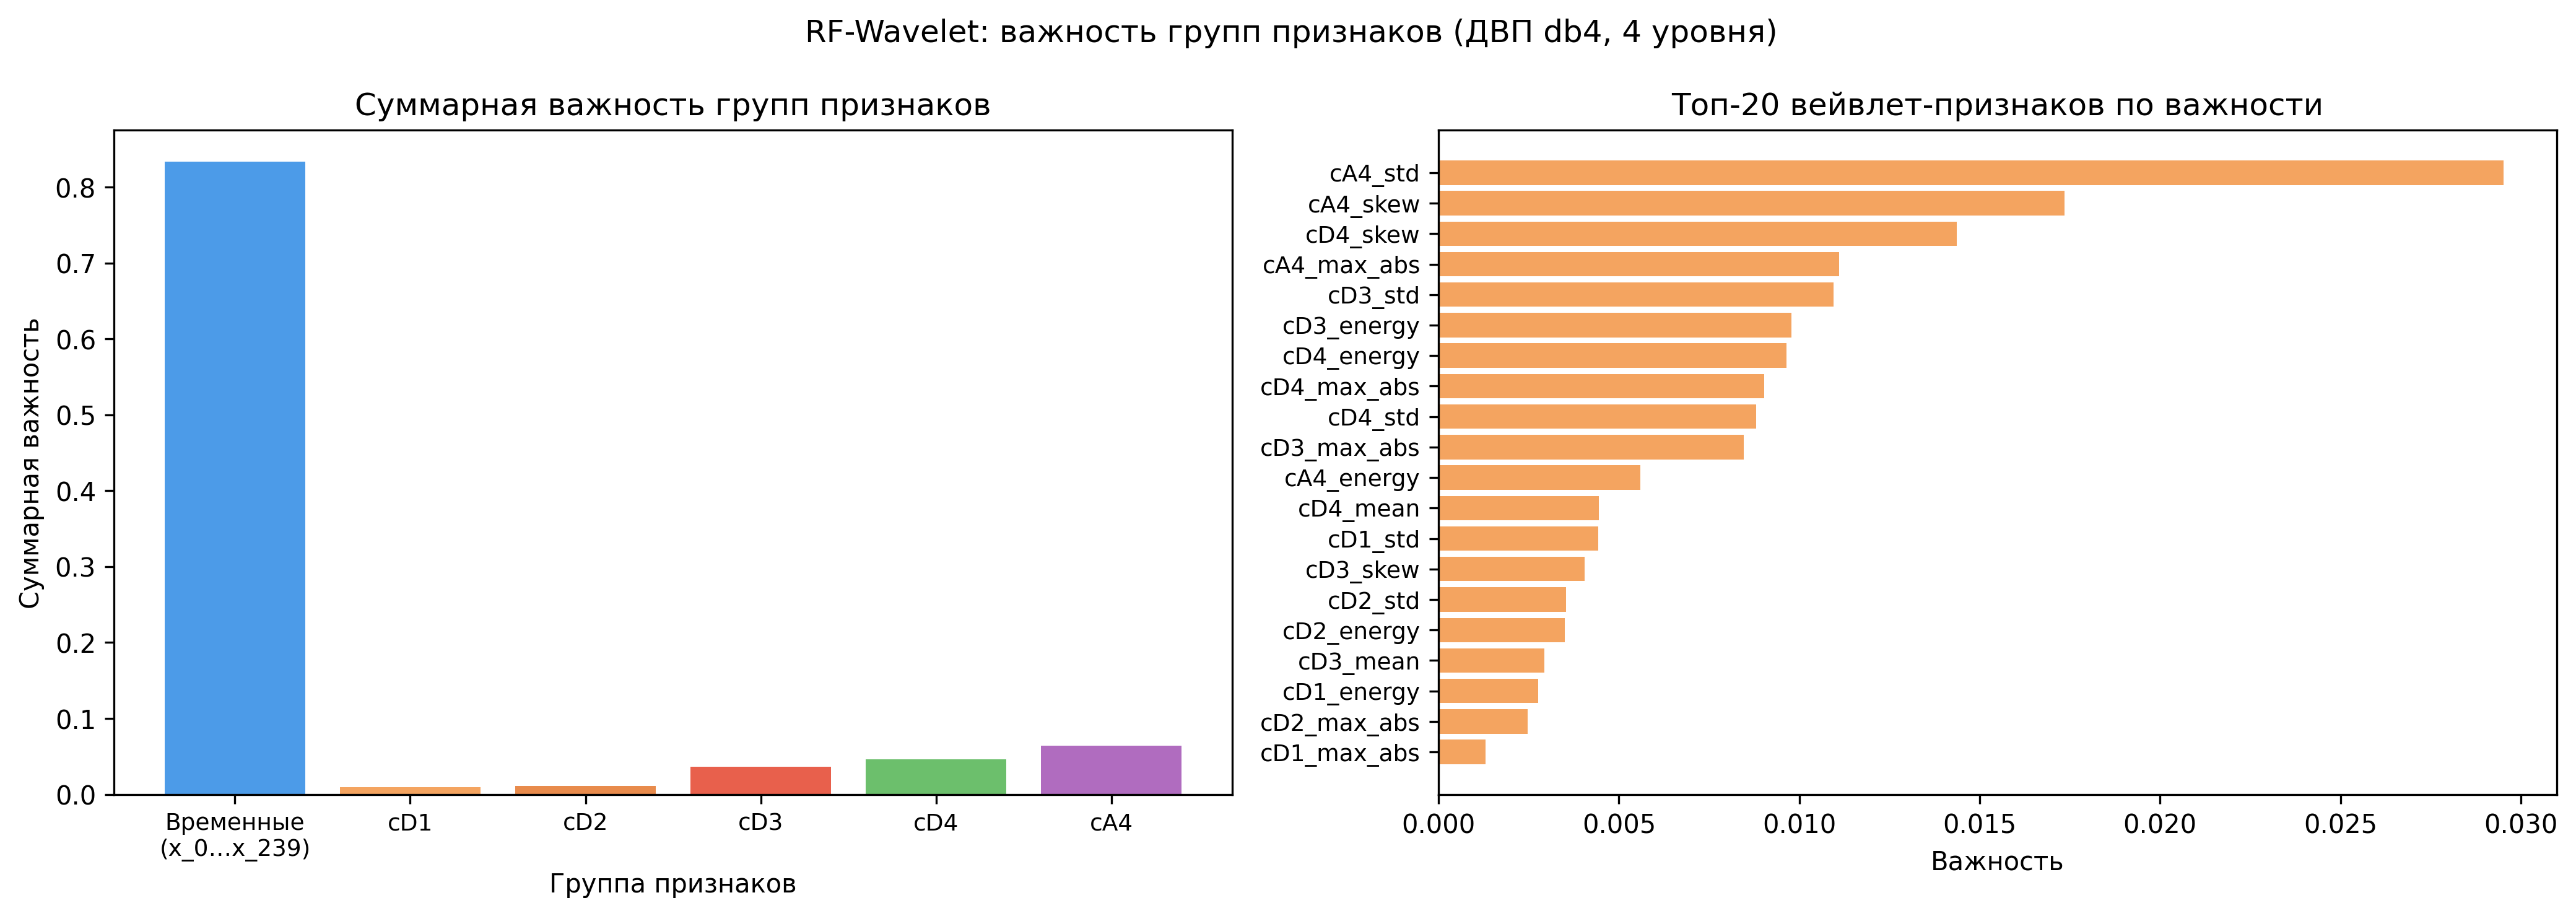
\includegraphics[width=\textwidth]{../reports/figures/models/rf_wavelet_feature_importance.png}
\caption{Важность групп признаков в~RF-Wavelet (слева~---
суммарно по~группам, справа~--- топ-20 вейвлет-признаков).}
\label{fig:wt_imp}
\end{figure}
